\section{Open Biomedical Ontology~(OBO)} Most biomedical ontologies are semantically rich and contain tens of thousands of classes. Managing these is expensive and often requires expert knowledge. The Open Biomedical Ontologies~(OBO)~Foundry\footnote{\url{http://obofoundry.org/} accessed 2018/05/21}, a community of experienced ontology developers and engineers for biomedical environments, manages many specialised biomedical ontologies. These are available in various formats, including the OBO~format, which was originally developed as part of the Gene Ontology~(GO)\footnote{\url{http://www.geneontology.org/} accessed 2018/05/21}. 

The OBO File Format Specification~1.2~\footnote{\url{https://owlcollab.github.io/oboformat/doc/GO.format.obo-1_2.html} accessed 2018/05/22} defines a flat document structure for OBO files. A file contains a header and one or more \emph{stanzas}. A stanza is a labeled section of a document, indicating that an object of a particular type is being described. Currently, there are three supported types: \textit{Term}, \textit{Typedef} and \textit{Instance}. Every stanza starts with an id-tag and an unbounded list of tag-value pairs. Looking at the supported tags, it is clear that the definition of meta-data is important to achieve the goals of \textit{readability}, \textit{ease of parsing}, \textit{extensibility} and \textit{minimal redundancy}. In particular, it allows, among others, the specification of 
\begin{inparaenum}[1)]
		\item the term definition (\texttt{def}),
		\item comments (\texttt{comment}),
		\item editorial data~(\texttt{is\_obsolete}, \texttt{replaced\_by}, \texttt{created\_by}, \texttt{creation\_date}) and
		\item cross references (\texttt{xref})
\end{inparaenum}.

Although the Open Biomedical Ontologies and Semantic Web representation languages have overlapping objectives, they evolved independently. To bring these two communities together, researchers have created a tool for converting OBO~ontologies to OWL and vice-versa without loosing any information during the conversion process~\cite{tirmizi2011}. It turned out that the majority of the OBO~vocabulary fits nicely into the Semantic Web Layer Cake. The mapping between the OBO Layer Cake and the Semantic Web Layer Cake is shown in~\hyperref[fig:semantic_obo_cake]{Figure~\ref*{fig:semantic_obo_cake}}. 

\begin{figure}
	 \centering
	 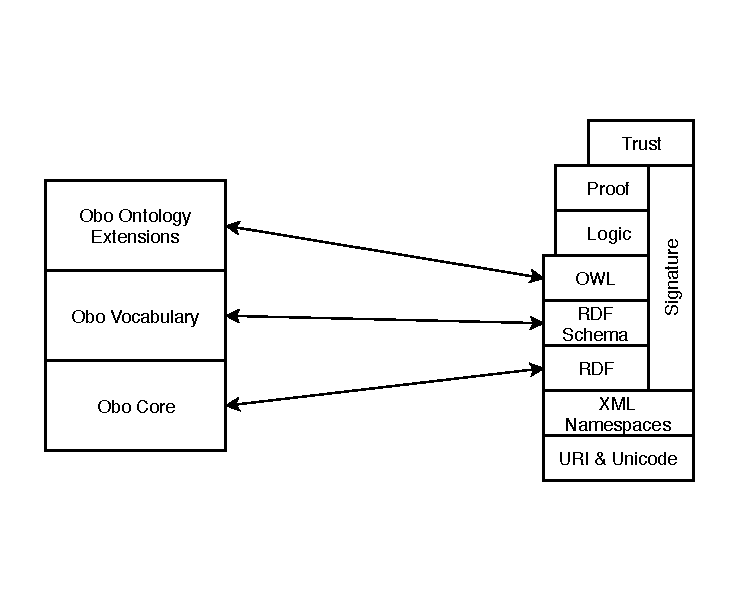
\includegraphics[width=0.5\textwidth]{drawio/Obo2Owl}
	 \caption{Mapping between OBO and the Semantic Web (depicted from~\cite{tirmizi2011})}\label{fig:semantic_obo_cake}
\end{figure}

\emph{OBO~Core} forms the bottom layer of the OBO Layer Cake. It mainly handles the assignment of ids and namespaces to RDF related concepts. Historically, OBO identifiers were limited in scope (local identifiers) while OWL requires global identifiers (URIs). This imposes some challenges on the translation process, e.g. URIs need to be prepended with prefixes. 

The next layer represents the \emph{OBO Vocabulary} which is mapped to RDF-Schema. As there exists a replacement for each of the terms in RDF-Schema, the translation process is implemented by replacing \texttt{names} with RDFS labels, \texttt{definitions} with RDFS labels, \texttt{comments} with RDFS comments, \texttt{is\_a} with subclass relations, \texttt{domains} with RDFS domain restrictions and \texttt{ranges} with RDFS range restrictions. 

The top most layer is represented by the \emph{OBO Ontology Extensions} which are mapped to OWL. Besides the definition of concept-level mappings, this layer defines tags for expressing meta-data on the entire ontology. For example, editorial meta-data (\texttt{creation\_date}, \texttt{replaced\_by} and \texttt{saved\_by}) is mapped to annotation properties. 

A summary of the most important OBO tags together with their OWL equivalents is given in~\hyperref[app:obo_terms]{Appendix~\ref*{app:obo_terms}}. However, for some OBO vocabulary there is no corresponding OWL tag. Therefore, a dedicated OWL namespace\footnote{http://www.geneontology.org/formats/oboInOwl\#} containing all OBO definitions was created. Furthermore, a recommended practice to preserve compatibility between OBO features and OWL features is to restrict editing of mapped OBO tags. A more detailed discussion on this topic is given in~\cite{tirmizi2011, tirmizi2006}.
